\documentclass[a4paper, 12pt]{article}

%%%%%%%%%%%%%%%%%%%%%%%%%%%%%%% PACKAGES %%%%%%%%%%%%%%%%%%%%%%%%%%%%%%%
% Math-related things
\usepackage{amsmath}
\usepackage{amssymb}
\usepackage{amsthm}
% Italian spelling
\usepackage[italian]{babel}
% Accenti e caratteri speciali
\usepackage[utf8]{inputenc}
% Margini e grafica della pagina
\usepackage[top=2cm, bottom=2cm, left=2cm, right=2cm]{geometry}
\usepackage{fancyhdr}
% Tabelle
\usepackage{tabularx}
% Graphs and Images handling
\usepackage{graphicx}
\usepackage{svg}
% VHDL language support
\usepackage{minted}
% Hypertext references
\usepackage{hyperref}

% Title Page
\title{Eriantys - Prova Finale di Ingegneria del Software}
\author{
	Paolo Pertino [10729600]
	\href{mailto:paolo.pertino@mail.polimi.it}{paolo.pertino@mail.polimi.it} \\
	Leonardo Pesce [10659489]
	\href{mailto:leonardo.pesce@mail.polimi.it}{leonardo.pesce@mail.polimi.it} \\
	Alberto Paddeu [10729194]
	\href{mailto:alberto.paddeu@mail.polimi.it}{alberto.paddeu@mail.polimi.it} \\
} 

% Contents page settings
\renewcommand*\contentsname{Indice}
\setcounter{tocdepth}{3}

\newcommand{\quantities}[1]{%
	\begin{tabular}{@{}c@{}}\strut#1\strut\end{tabular}%
}

% General page settings
\pagestyle{fancy}
\fancyhf{}
\rhead{\leftmark}
\lhead{Eriantys - Prova Finale di Ingegneria del Software}
\cfoot{\thepage}

% Hyperrefs setup
\hypersetup{
	colorlinks=true,
	linkcolor=[rgb]{0.996,0.396,0.090196}, %254 101 23
	filecolor=magenta,      
	urlcolor=[rgb]{0.72156862745,0.0078431372549,0.00392156862745},
	citecolor=[rgb]{0.517647,0.0156862745,0.0117647},
	pdftitle={Eriantys - Prova Finale di Ingegneria del Software},
	pdfpagemode=FullScreen,
}

\begin{document}
	\pagenumbering{gobble}
	\date{\today}
	\maketitle
	\newpage
	\pagenumbering{arabic}
	
	\tableofcontents
	
	\newpage
	\section{Introduzione}
	\paragraph{}
	La \textbf{Prova Finale di Ingegneria del Software} dell'anno scolastico 2021-2022 prevede lo sviluppo di una versione software del gioco da tavolo \emph{Eriantys}, un prodotto \emph{Cranio Creations}\cite{eriantys} che si ispira e tenta di rinnovare il già affermato \emph{Carolus Magnus}\cite{carolusMagnus}.
	
	\paragraph{}
	Il prodotto finale dovrà soddisfare i requisiti \emph{Game-Specific} e \emph{Game-Agnostic} indicati nel documento \emph{requirements.pdf}. In particolare è richiesto l'utilizzo del design pattern \emph{Model-View-Controller} di cui a breve forniremo una concisa descrizione.\\
	Per incrementare il punteggio ottenuto, il team si concentrerà nell'implementazione delle regole complete del gioco, nel fornire la possibilità ai giocatori di connettersi al server e giocare tramite un'interfaccia a linea di comando (CLI) oppure mediante l'interazione con un'interfaccia grafica (GUI). Infine si darà spazio all'implementazione di quante più possibili delle seguente funzionalità aggiuntive: \emph{12 carte personaggio, partite a 4 giocatori, partite multiple e persistenza}.
	
	\subsection{Model-View-Controller}
	\paragraph{}
	Il \emph{Model-View-Controller} è un design pattern per la progettazione di un'architettura software. Esso permette di separare la logica di presentazione dell'applicativo da quella applicativa(o detta di business).\\
	\begin{figure}[h!]
		\centering
		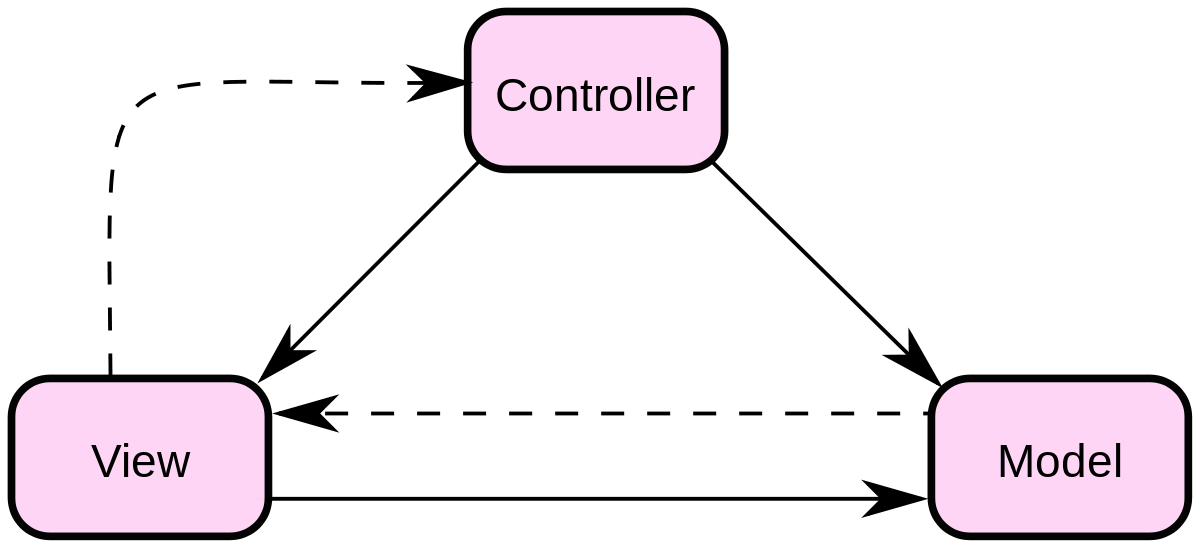
\includegraphics[scale=0.35]{mvc.png}
		\caption{Model-View-Controller Pattern}
	\end{figure}
	
	Come deducibile dal nome, tale architettura è strutturata su 3 differenti layer:\\
	\begin{enumerate}
		\item \emph{Model} - gestione diretta dei dati, della logica e delle regole del programma. Si noti come l'utente non modifica in modo diretto lo stato del model, bensì si interfaccia con il controller il quale gestisce in separata sede l'interazione con lo stato interno del sistema;
		\item \emph{View} - permette la visualizzazione dello stato del model e gestisce l'interazione con gli utenti e agenti esterni; 
		\item \emph{Controller} - riceve i comandi dell'utente attraverso la view e li attua modificando gli stati degli altri due layers.
	\end{enumerate}
	Sono possibili viste multiple di uno stesso modello. Nel nostro caso, infatti, saranno implementate due viste: il gioco sarà pertanto accessibile sia attraverso linea di comando sia mediante interfaccia grafica.
	
	\newpage
	\section{Devlog}
	\paragraph{}
	Nella seguente sezione riportiamo settimana per settimana i progressi effettuati dal team, evidenziando, ove necessario, eventuali diagrammi e gli snodi del ragionamento.
	\subsection{Settimana 1: Un primo sguardo al class diagram del Modello}
	\paragraph{}
	Durante la prima settimana di corso abbiamo analizzato i componenti fisici del gioco e le sue regole, cercando di riprodurre uno schema logico di tali elementi attraverso un \emph{Class Diagram UML}. Esso contiene una prima bozza della struttura del Model:\\
	\begin{figure}[h]
		\centering
		\def\svgwidth{\columnwidth}
		\resizebox{\linewidth}{!}{\input{umlFirstWeek.pdf_tex}}
		\caption{Class Diagram del Model - Bozza}
	\end{figure}\\
	Come indicato, lo schema sopra riportato è una bozza primitiva e di seguito riportiamo i principali ragionamenti effettuati:\\
	\begin{itemize}
		\setlength{\parskip}{0pt}
		\setlength{\parsep}{0pt}
		
		\item Tutti i componenti fisici, in futuro, avranno una loro grafica che dovrà essere mostrata. Pertanto implementano l'interfaccia GameObject che prevede l'implementazione di un metodo specifico per conseguire tale obiettivo.
		\item Il cerchio di isole che costituisce la board di gioco è stato pensato come \emph{Doubly Circular Linked List}\cite{circularDoublyLinkedList}. Con tale rappresentazione sarà più agevole lo spostamento di madre natura e l'operazione di merge di 2 isole consecutive a valle della loro conquista da parte di un giocatore.
		\item Volendo implementare le regole complete, quindi prevedendo la possibilità di giocare una partita seguendo la modalità per esperti, e tenendo conto della possibilità di implementare partite multiple sullo stesso server, ci siamo interrogati su come far impattare tale scelta sui diversi metodi delle varie classi. L'idea è quindi quella di utilizzare un Template Pattern creando una classe astratta di gioco dalla quale saranno derivate le 3 versioni di gioco (per 2, 3 e 4 giocatori). Da esse discenderanno successivamente le corrispettive versioni a 2, 3 e 4 giocatori in modalità per esperti.
		\item In vista dell'implementazione della funzionalità di persistenza della partita, è stato brevemente analizzato il pattern \emph{Memento} ed il suo funzionamento per capire se esso possa essere utile in futuro.
	\end{itemize}
	
	% Strumenti usati
	\newpage
	\section{Strumenti utilizzati}
	Nella seguente sezione verranno indicati i principali strumenti di sviluppo utilizzati:\\
	\begin{itemize}
		\setlength{\parskip}{0pt}
		\setlength{\parsep}{0pt}
		
		\item \emph{IntelliJ IDEA Ultimate 2021.3.2} - Principale IDE utilizzato.
		\item \emph{Maven} - Gestione dello sviluppo del progetto software e di tutte le sue fasi.
		\item \emph{JUnit} - Framework principale di unit testing.
		\item \emph{AstahUML} - Creazione di diagrammi UML.
		\item \emph{GitKraken} - Git GUI per visualizzare il workflow di sviluppo ed utilizzare efficientemente Git.
		\item \emph{TEXStudio} - Gestione e aggiornamento del report.
	\end{itemize}
	% Bibliografia
	\newpage
	\begin{thebibliography}{99}
		\bibitem{eriantys}
		\href{https://www.craniocreations.it/prodotto/eriantys/}{Eriantys, Cranio Creations}
		
		\bibitem{carolusMagnus}
		\href{https://www.goblins.net/giochi/carolus-magnus-5071}{Carolvs Magnvs, Winning Moves}
		
		\bibitem{circularDoublyLinkedList}
		\href{https://www.softwaretestinghelp.com/doubly-linked-list-in-java/#Circular_Doubly_Linked_List_In_Java}{Circular Doubly Linked List}
		
	\end{thebibliography} 
\end{document}         
